\documentclass[dvisvgm,multi=true]{standalone}
\usepackage{mathmlcoresvg}
\begin{document}
%<figcaption><span>Figure 12: </span>Box model for the <code>mroot</code> element</figcaption>
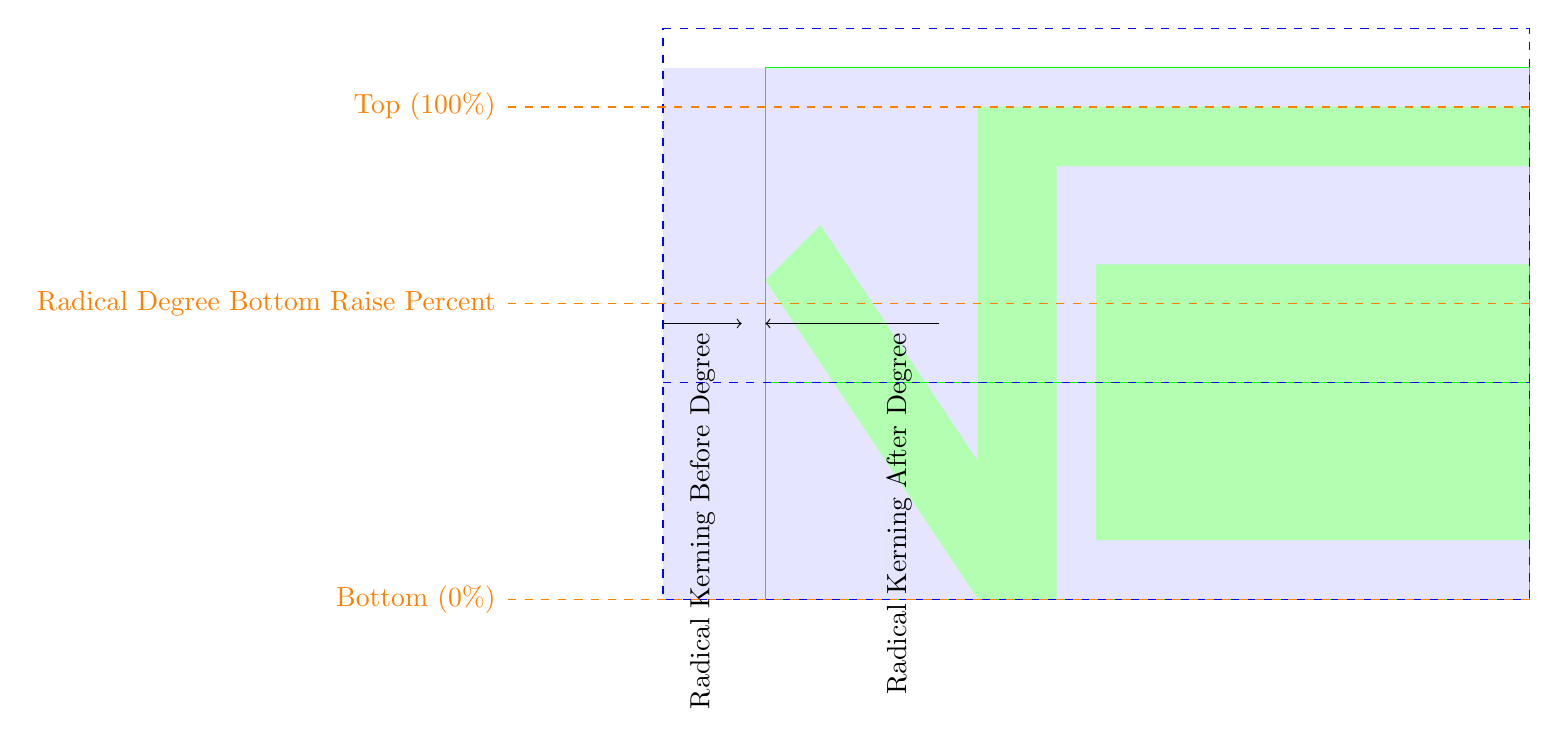
\begin{tikzpicture}[yscale=-1]
  \fill[blue!10] (0,-3) -- (11,-3) -- (11,3.75) -- (0,3.75) -- cycle;

  \begin{scope}[shift={(6,0)}]
  \fill[green!30]
  (5,-2.5) -- (-2,-2.5) -- (-2,2) --
  (-4,-1) -- (-4.7,-.3) -- (-2.7,2.7) -- (-2,3.75) -- (-1,3.75) --
  (-1,-1.75) -- (5,-1.75) -- (5,-2.5)
  (-.5,-.5) -- (5,-.5) -- (5,3) -- (-.5,3) -- cycle;
  \draw[green] (-4.7,-3) -- (5,-3) -- (5,3.75) -- (-4.7,3.75) -- cycle
  (-4.7,1)--(5,1);
  \end{scope}

  \MathMLBox{1}{-1.5}{.5}{1}{red}

  \draw[dashed,blue] (0,-3.5) -- (11,-3.5) -- (11,3.75) -- (0,3.75) -- cycle
  (0,1)--(11,1);

  \draw[dashed,orange](11,3.75)--(-2,3.75) node[left]{Bottom (0\%)};
  \draw[dashed,orange](11,0)--(-2,0) node[left]
       {Radical Degree Bottom Raise Percent};
  \draw[dashed,orange](11,-2.5)--(-2,-2.5) node[left]{Top (100\%)};

  \draw[->,black] (0,.25) -- (.5,.25) node[left,rotate=90]
       {Radical Kerning Before Degree} -- (1,.25);
  \draw[->,black] (3.5,.25) -- (3,.25) node[left,rotate=90]
       {Radical Kerning After Degree} -- (1.3,.25);
\end{tikzpicture}

\end{document}
